\subsubsection{Trigger System}
\label{sec:tesrun_trigger}

A block diagram of the HPS test run trigger processing is shown in Figure \ref{fig:trigger_diagram}.  A gigabit bandwidth is used to transport all the individual FADC250 channel sums (5-bits) and clock (3-bits) encoding bits to resolve a $4$ ns period within a $32$ ns frame.  The clock encoding bits report the time when the input signal crosses the programmable threshold within the $32$ ns frame.  If the input signal does not cross threshold for a given $32$ ns frame, then the channel data is reported as zero.

\begin{figure}[t]
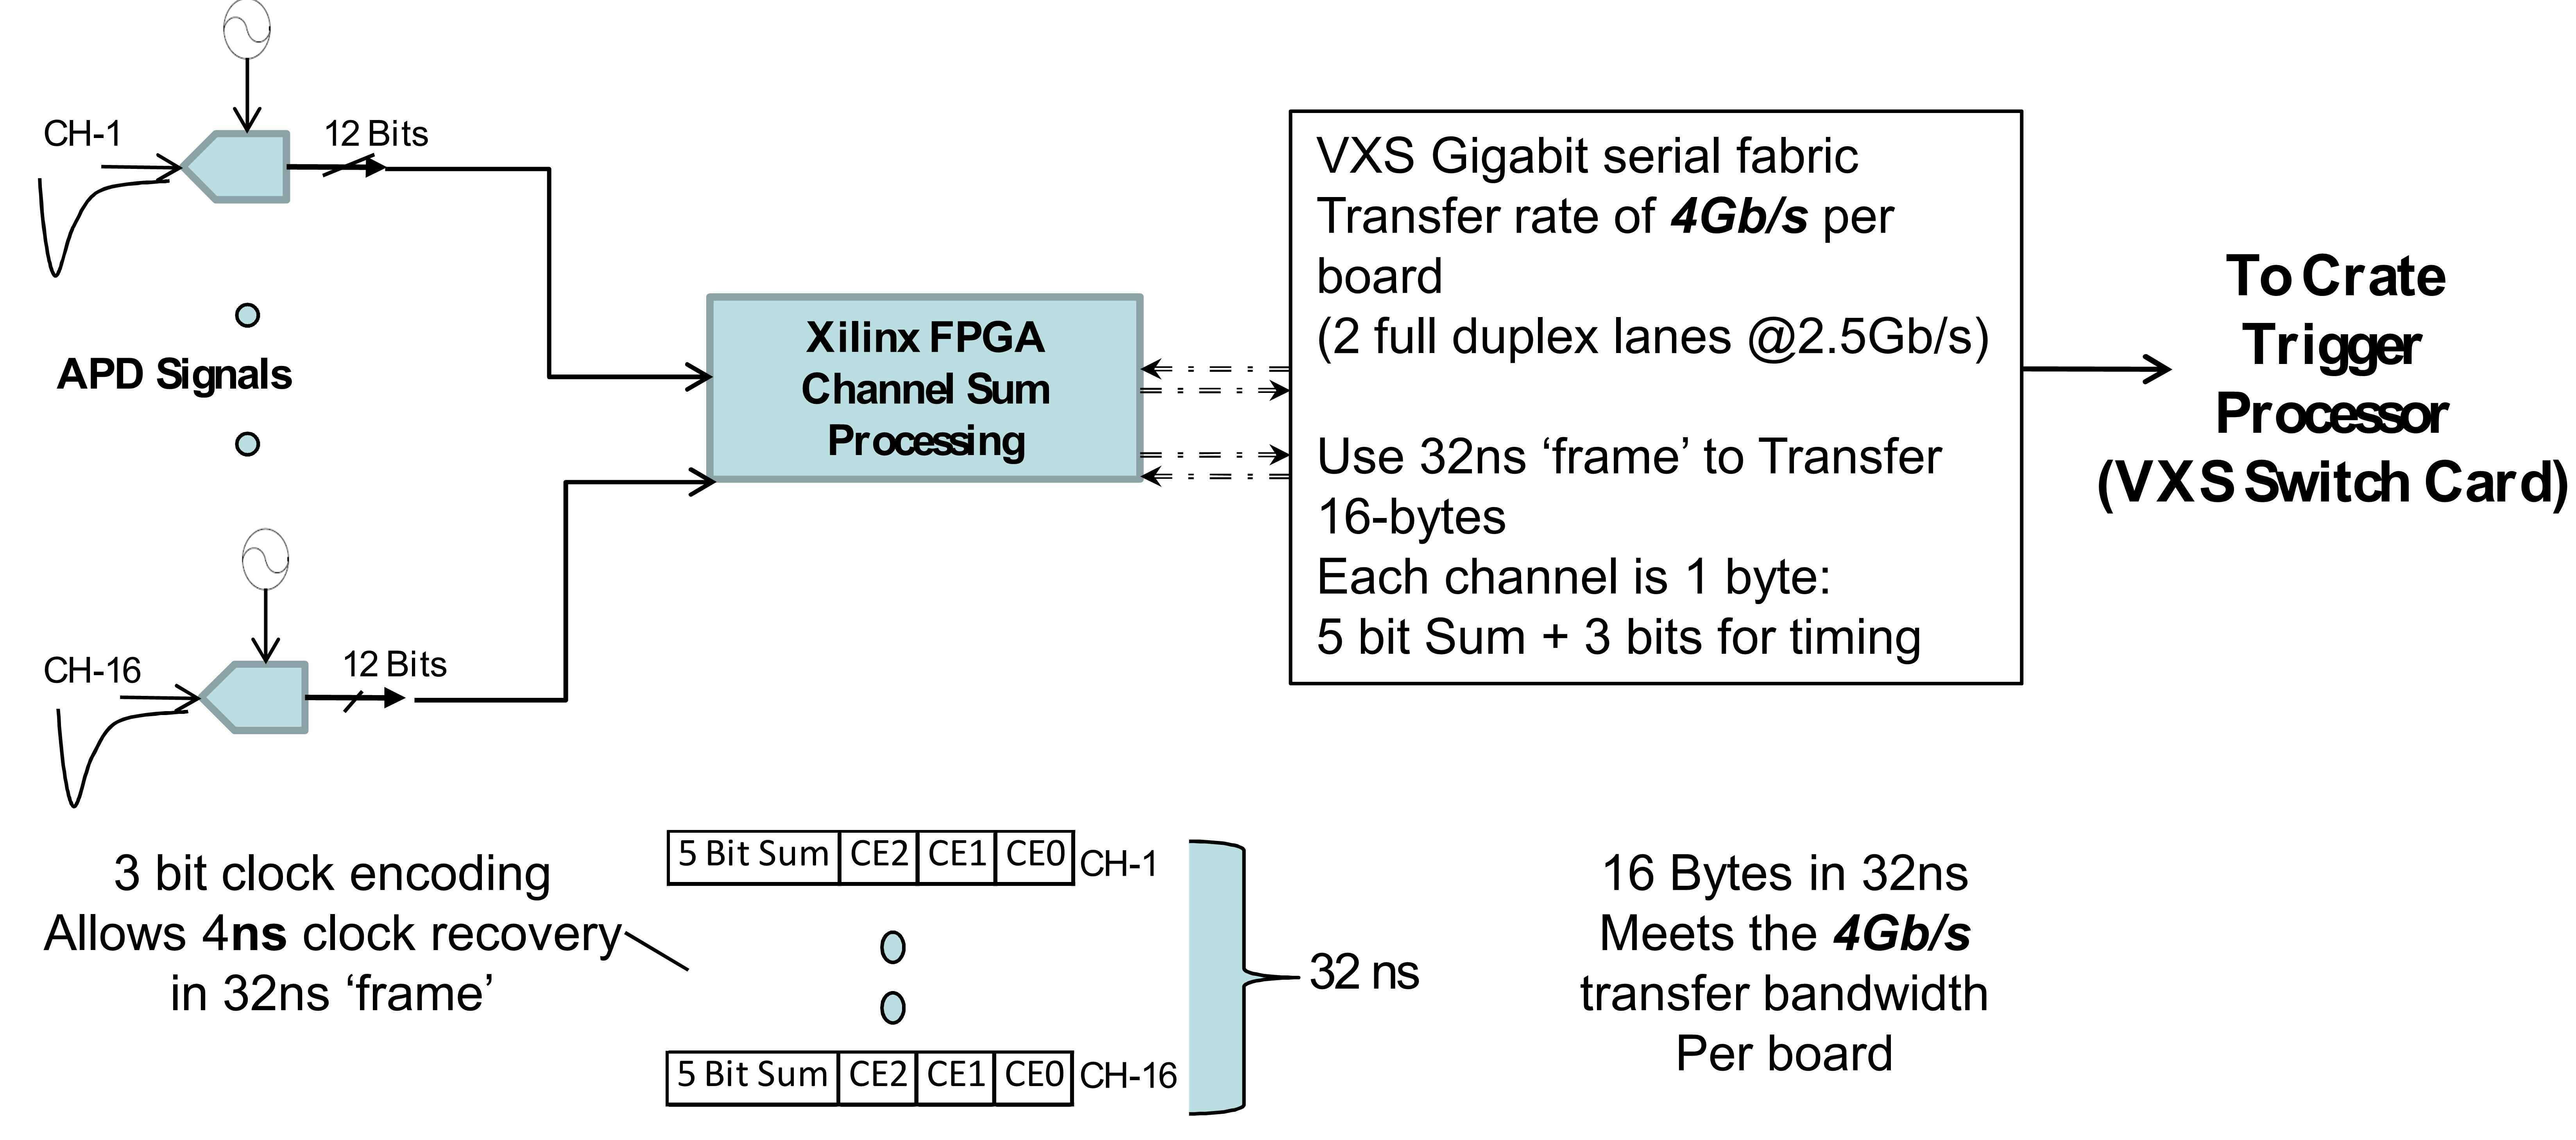
\includegraphics[scale=0.6]{test2012/trigger/HPSChanSum_001.jpg}
\caption{\small{Block diagram for the trigger system.}}\label{fig:trigger_diagram}
\end{figure}

The reported 5-bit channel sum value is extracted from the 17-bit register that contains the integrated (sum) signal value of the input channel.  The channel integration occurs only if the input signal crosses the programmable threshold level.  The samples that are included in the channel integration are those that are above threshold.  The number of samples for a given channel integration will not be larger than the frame report latency time (MAX=128ns or 32 samples). Samples of the input signal are shown in Figure \ref{fig:trigsamples}. The point where the input signal crosses threshold determines which frame the integrated value is reported.  The time where the input signal crosses threshold is captured within the frame and reported with the three clock encoding bits to a 4ns time stamp of the threshold crossing time.

\begin{figure}[t]
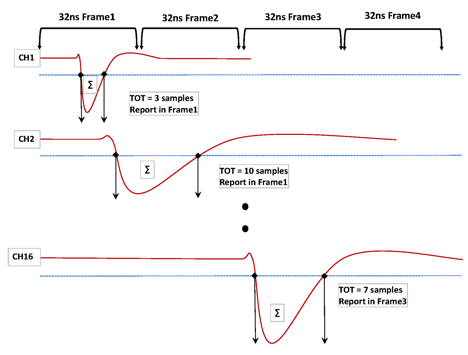
\includegraphics[scale=0.9]{test2012/trigger//trigger_pulse_samples}
\caption{\small{Example of input signals, and how they are integrated for the test run trigger.}}\label{fig:trigsamples}
\end{figure}

In the example, the pulse for channel 2 crosses multiple frames.  The point where the signal crosses threshold determines the frame where the integration value will be reported for the given channel.  The number of points that are over threshold will be limited to 32. If multiple pulses within a 32 ns frame they will not be resolved will crate pile-up effect.  The trigger application will only process a single falling edge or single rising edge per 32ns frame.  Multiple pulse signals may be recoverable from the readout data offline.

Information from each FADC channel were reported to the Crate Trigger Processor (CTP) through Gigabit serial data streams. The sixteen serial data streams will be processed on a frame by frame basis, and the cluster finding algorithm (the same as described in \ref{sec:triggerdaq} for HPS) will produce a serial data stream that will be processed by the Sub-System Processor (SSP) to create a readout trigger signal that can be distributed to the front end FADC250 for Physics event readout. The system was designed for maximum trigger accept rate of 50 KHz. 

For the test run, the trigger decision in the SSP was a simple threshold: the trigger would fire on a single cluster with energy exceeding the threshold. The full trigger described in \cite{HPS_tPROP} was implemented, and the cluster pair trigger was tested.
